\newpage
\subsection*{Question 5}

\subsubsection*{Part E - Questions}
\begin{enumerate}
    \item In \textit{part E}, we need to generate a coverage report on the apache-commons-io project using two different code coverage tools, JaCoCo and OClover so we can compare how the project is covered by each. We are looking for differences in code coverage, or in other words, if the code coverage tools do not cover the project code in an identical way. In case of difference in code coverage, we must understand why the code coverage tools behave differently. 
    \item  In order to do so, we duplicate the project folder and modify pom.xml file for each so we can use JaCoCo for one and OClover for the other. We then need to modify pom.xml file to make the plugin work. For JaCoCo, we need to specify the JaCoCo version in the \textit{properties} as well as add the JaCoCo plugin in the \textit{plugins} section. For clover, we have to add the plugin in the \textit{plugins} section. \\ Running the command \verb|mvn test| will automatically generate coverage results in an .xml format for OClover and .csv for JaCoCo. These report files can then be analyzed to try and notice differences between the code coverage tools under study. 
    \item 
    \begin{center}
        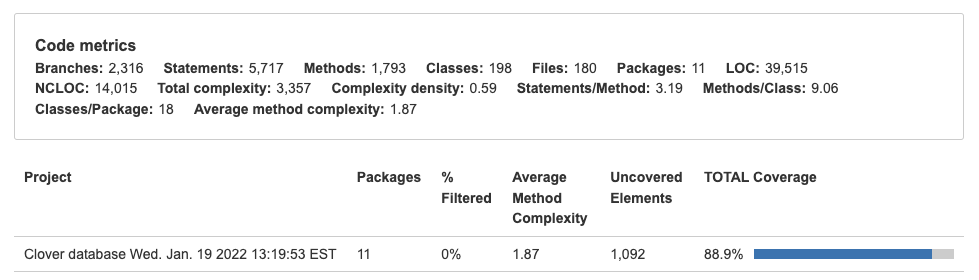
\includegraphics[width=0.9\textwidth]{img/clover1.png}
    \end{center}
    \begin{center}
        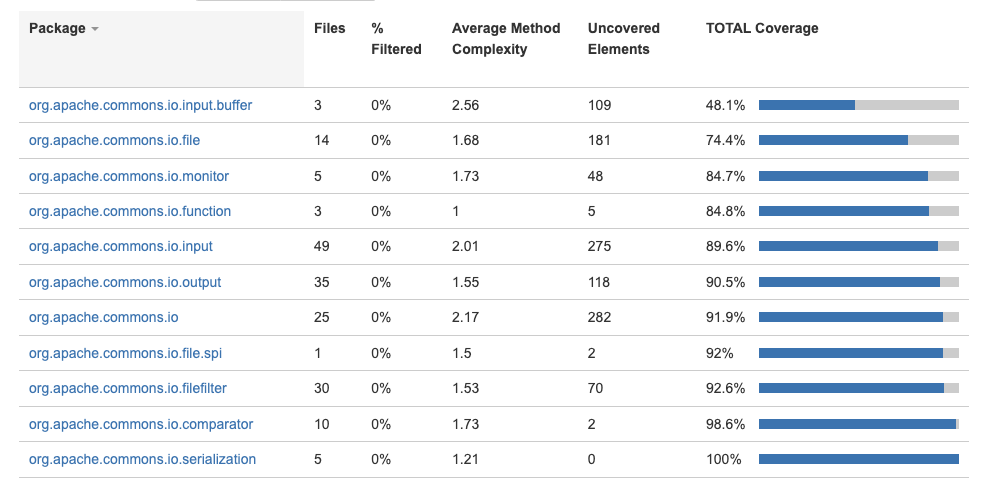
\includegraphics[width=0.9\textwidth]{img/clover2.png}
    \end{center}
    \noindent Tables above show code coverage of the project using OClover. Metrics like the number of statements, branches methods, classes in the project as well as more interesting ones like number of uncovered elements per package and total coverage percentage can be easily viewed.
    \begin{center}
        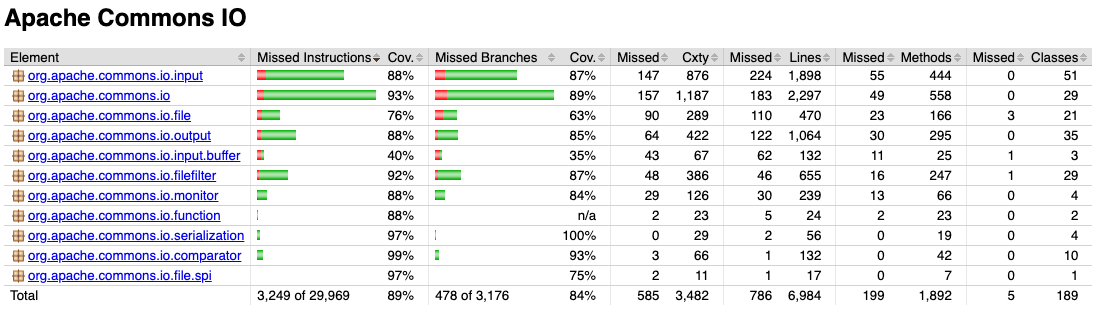
\includegraphics[width=1\textwidth]{img/jacoco1.png}
    \end{center}
    \noindent In the table above we can see an overview of the project coverage as presented by JaCoCo. Both tools offer a way to easily view approximately the same metrics. 
    
    \item 
        \begin{enumerate}[label={\alph*)}]
            \item Yes, when analyzing the results presented by each tool, we can clearly see that for many files, the number of covered statements is not the same when using JaCoCo compared to when using OClover.\\ A script is used to compile the project's statement coverage obtained with each tool. Both the script (\textit{script.ipynb}) and the compiled results (\textit{report.txt}) are joined with this report. By looking at the compiled results, it is obvious that JaCoCo and OClover have different ways to compute metrics since coverage results differ for a majority of files.
        \end{enumerate}
\end{enumerate}

\subsection*{Question 5 -  Questions}
\begin{enumerate}[label={\alph*)}]
    \item Yes, when analyzing the results presented by each tool, we can clearly see that for many files, the number of covered statements is not the same when using JaCoCo compared to when using OClover.\\ A script is used to compile the project's statement coverage obtained with each tool. Both the script (\textit{script.ipynb}) and the compiled results (\textit{report.txt}) are joined with this report. By looking at the compiled results, it is obvious that JaCoCo and OClover have different ways to compute metrics since coverage results differ for a majority of files.\\
    \begin{center}
        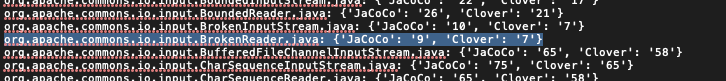
\includegraphics[width=0.8\textwidth]{img/brok.png}
    \end{center}
    For example, the \verb|org.apache.commons.io.input.BrokenReader| file has 9 statements covered when analyzed using JaCoCo and only 7 with OClover. This file has 8 'methods' including constructors. If we take a closer look at the \verb|BrokenReader(IOException)| constructor, we see that in JaCoCo, all three lines of the method are counted as covered methods whereas using OClover, only the header and the statement are (not the final closing curly-bracket).
    \begin{center}
        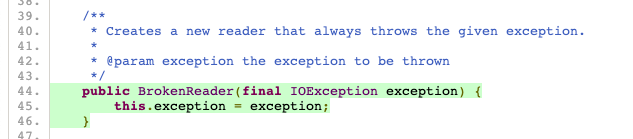
\includegraphics[width=1\textwidth]{img/jccex.png}
    \end{center}
    \noindent Above is line coverage for the \verb|BrokenReader(IOException)| constructor using JaCoCo.
    \begin{center}
        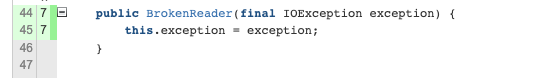
\includegraphics[width=1\textwidth]{img/cloex.png}
    \end{center}
    \noindent Above is line coverage for the \verb|BrokenReader(IOException)| constructor using OClover.\\
    \noindent These results show that while OClover only counts statements, JaCoCo tends to count lines of code based on the actual source lines. For example, if a method ends because a \verb|return| statement or a \verb|throw| statement is reached, the final closing curly bracket is not counted as a line (since the execution never reached it) however, if the method is completely executed and the final closing curly bracket is reached, then it is counted as a covered line by JaCoCo. OClover does not operate this way. OClover counts the number of statement that have been executed through a test run.
    \noindent Let's cover another example using the \verb|../org.apache.commons.io.comparator.NameFileComparator| file. While analysis with both tools return a $100\%$ test coverage, we see that the number of covered lines/statements differ:
    \begin{center}
        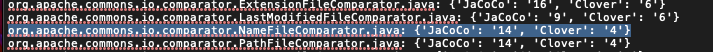
\includegraphics[width=0.8\textwidth]{img/mani.png}
    \end{center}
    
    \noindent This difference is due to the fact that JaCoCo counts the class variables initialization lines as covered lines because statements are executed (namely \verb|new| statement), while OClover only counts the statements associated with methods. 
    
    \begin{center}
        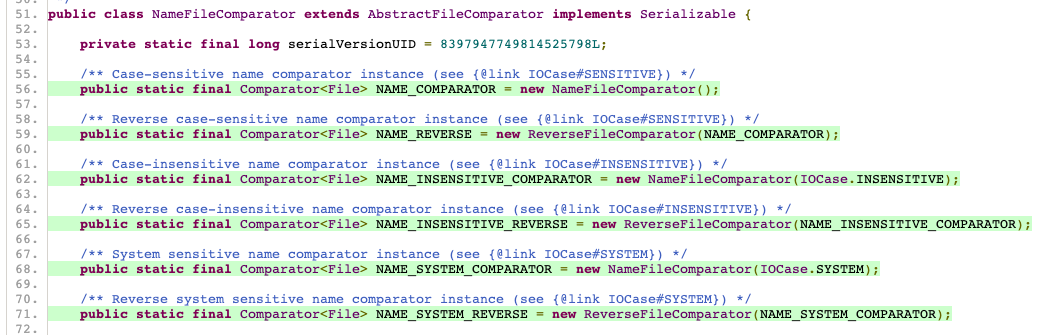
\includegraphics[width=1.1\textwidth]{img/fieldJ.png}
    \end{center}
    \noindent Class variable initialization are counted as line covered when using JaCoCo as seen in the picture above. 
    
    \begin{center}
        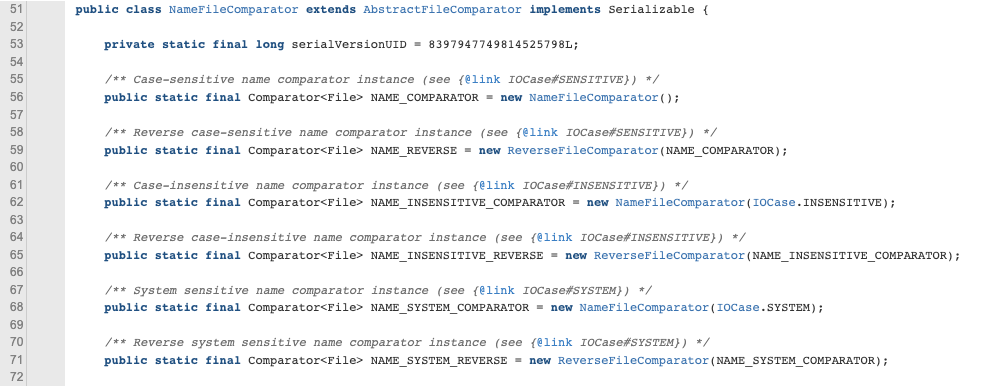
\includegraphics[width=1.1\textwidth]{img/fieldC.png}
    \end{center}
    \noindent Class variable initialization are not counted as statements covered when using OClover as seen in the picture above. \\
    
    \noindent Many of these differences come down to the way the source formatting is done. Indeed, a single line of a source code can refer to another class or another function with its own number of source lines that are going to be covered as well since it was invoked. Because of that, it is impossible to simply add the number of statements covered within a particular class. JaCoCo calculates line coverage based on the actual number of lines covered during the execution of tests. 
    
    \item The first file used for a) was \verb|org.apache.commons.io.input.BrokenReader| since all methods are simple with no decision points and no branch, each one has a cyclomatic ocmplexity of 1. If we follow the theory, CC =  B - D + 1 where B is the number of branches and D the number of decision points. Since the class has 8 methods a theoretical Cyclomatic complexity of 8 is expected. Both JaCoCo and OClover find that same answer. \\
    For the second file used in a), namely \\ \verb|../org.apache.commons.io.comparator.NameFileComparator| the tools return two different numbers when it comes to cyclomatic complexity. Indeed, JaCoCo finds a cyclomatic complexity of 6 while OClover finds 5. This is due to the fact that JaCoCo considers the class variables definitions as having a cyclomatic complexity of 1 while as previously stated, OClover does not consider these lines. The method \verb|NameFileComparator(IOCase)| is interesting since it includes an \verb|if| statement. Both JaCoCo and OClover find a cyclomatic complexity of 2 for this method as it contains a single if statement, allowing two branches. If we compute the theoretical cyclomatic complexity for this method we find: $CC = B - D + 1 = 2 - 1 + 1 = 2$. Hence, the values returned by both tools are equal to the theoretical value. 
    \begin{center}
        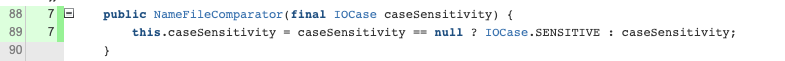
\includegraphics[width=1.1\textwidth]{img/method.png}
    \end{center}
    
    \noindent However, if we compute the theoretical cyclomatic complexity for this whole class, we obtain a value of 5. Only OClover returns the right value as JaCoCo's cyclomatic complexity takes into account the class variables.
    \item In order to have more meaningful results, I would suggest OClover over JaCoCo. Even though a lot of the metrics are similar, while completing part E, I realised that while OClover returns the number of statements covered by the tests, JaCoCo finds the number of lines covered which will make it count meaningless lines in term of code coverage like closing curly braces for example. This can boost the line coverage percentage and hide some issues. On the other side, OClover deals with executed (or missed) statements that express some action to be carried out by the program. I also prefer the OClover web interface which I think provides the user with more details. That being said, both tools are complete and seamless to use. 
    \item The metrics provided by both tools are in my opinion very complete. However, it would be even better if the tools provided the user with a user interface that would let the user chose what test to run, what folder to work on etc (even though additional plugins will let you do so). Also, it would be a good addition to allow the user to manipulate the metrics via the web-interface after the report is generated, to allow for an direct comparison and analysis of the data. 
\end{enumerate}